\chapter{Supplementary information to \texorpdfstring{\cref{sec:balancer}}{the balancer project}}
\label{sec:suppl_balancer}

\section{Mutational signature analysis}
\label{sec:suppl_mutsign}

Starting from the set of 520,521 balancer- or wild type-specific \acp{snv},
I removed the ones which are present in the DGRP freeze 2.0 \snv call set.
Then I used the R package \textsc{SomaticSignatures} \citep{Gehring2015} to
count base substitutions and their contexts of the remaining 58,457 variants
and plotted their relative frequencies in \cref{fig:signatures}. The absence
of striking differences between balancer and wild type spectra demotivated me
from deeper investigations of mutational signatures.

\begin{figure}[!ht]
  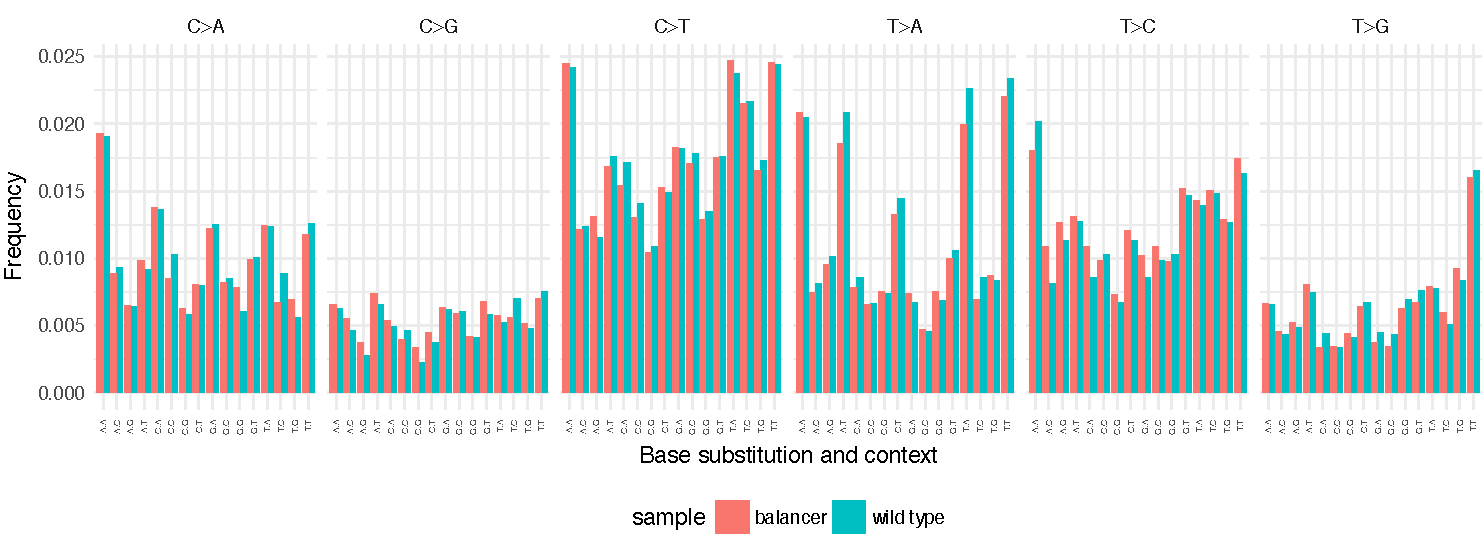
\includegraphics[width=\textplusmargin,inner]{snp_signatures_dgrp_removed.pdf}%
  \figcap{signatures}{\Ac{snv} mutation spectrum}{Frequency of the different
        base substitutions in their three-nucleotide context for balancer- and
        wild type-specific \acp{snv}. \Acp{snv} that are found in DGRP were
        removed, leaving 58,457 variants.}
\end{figure}
